\documentclass[a4paper]{article}
\usepackage[lmargin=2cm, rmargin=2cm]{geometry}
\usepackage{femape}
\usepackage{tikz}
\usetikzlibrary{graphs, graphdrawing, shapes}
\usegdlibrary{trees}
\disableindent
\title{Einführung in die Psychologie}
\author{Felix Leitl}
\begin{document}
\maketitle
\tableofcontents
\newpage
\section{Forschungsmethoden}
\section{Biologische Evolution}
\section{Wahrnehmung}
\subsection{Wahrnehmungsprozess}
Kein passiv abbildender, sondern aktiver, konstruierender Vorgang!
\begin{enumerate}
	\item Distaler Stimulus
	\item Transformation Licht
		\begin{enumerate}
			\item Fokussieren auf Retina
			\item Proximaler Stimulus
		\end{enumerate}
	\item Sensorische Prozesse am Rezeptor
		\begin{enumerate}
			\item Transduktion
			\item Neuronale Repräsentation 
		\end{enumerate}
	\item Neuronale Verarbeitung
	\item Wahrnehmung
	\item Erkennen
	\item Handlen
\end{enumerate}
\subsection{Sehen}
\subsubsection{Physik}
Spezifische Wellenlängen (380 - 780 nm) werden als verschiedene Farben wahrgenommen.

\subsubsection{Fokussieren auf der Retina}
Cornea und Linse (80/20\% fix/variabel) fokussieren Bild auf Retina (Netzhaut). Visuelle Rezeptoren auf der Netzhaut (Stäbchen und Zapfen) enthalten visuelle Pigmente \rightarrow Transduktion. Sehnerv leitet Informationen von Retina ans Gehirn weiter.

\subsubsection{Transduktion im Visuellen Rezeptor}
Durch auftreffen von Licht auf den visuellen Rezeptor gehen die Na$^+$ Kanäle zu \Rightarrow Zelle wird hyperpolarisiert und schüttet weniger Glutamat aus

\subsubsection{Neuronale Verarbeitung}
\begin{center}
	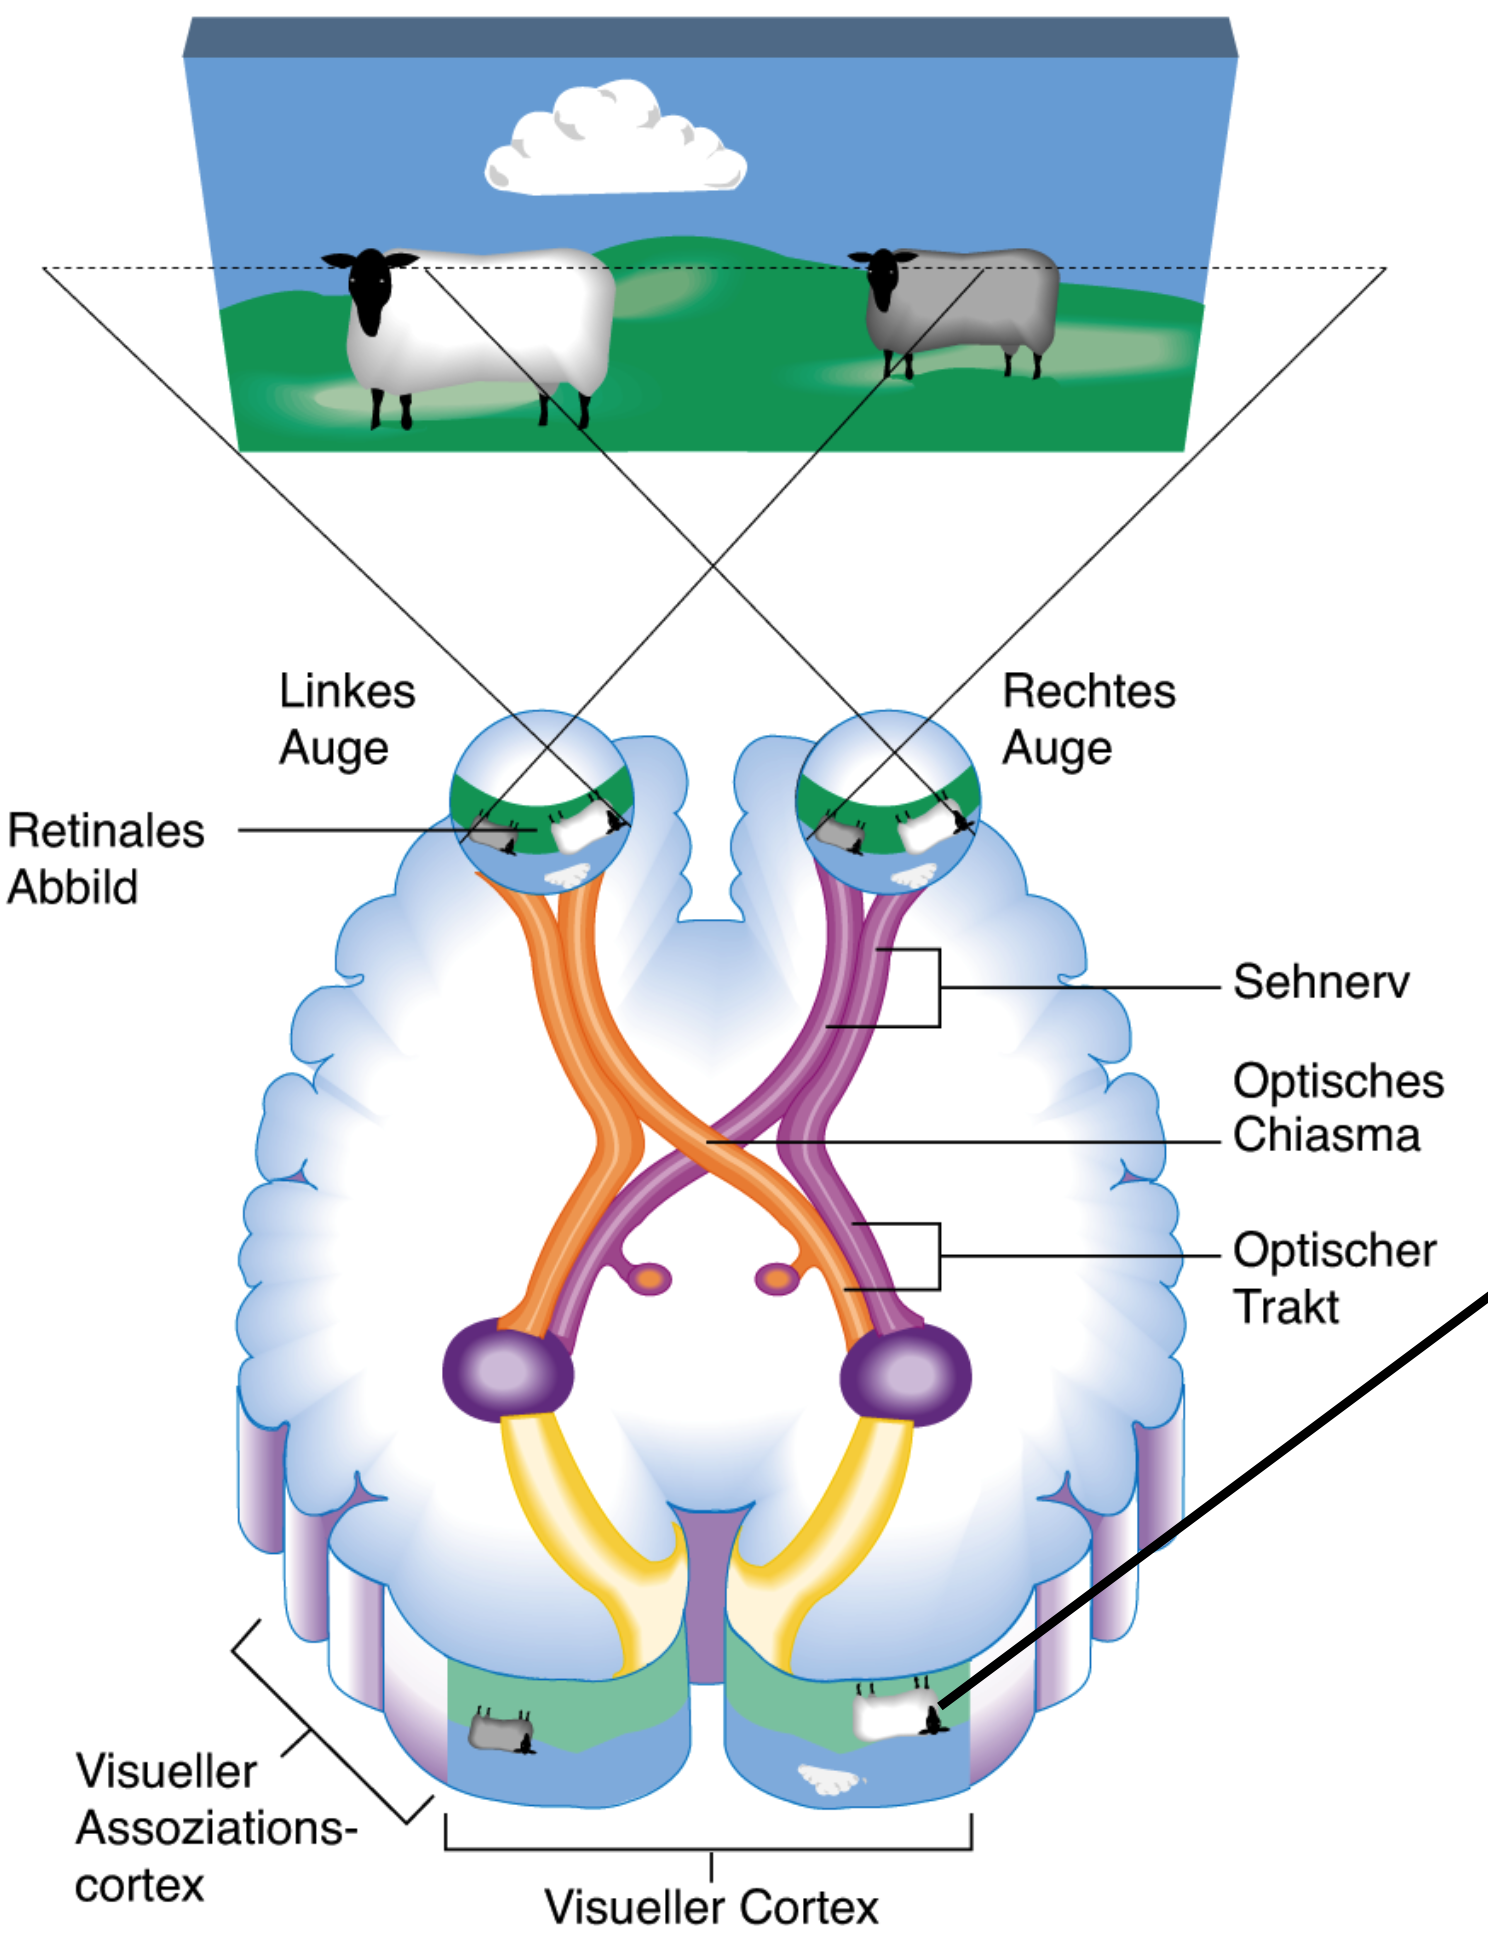
\includegraphics[scale=.2]{img/Auge.png}
\end{center}

\subsubsection{Verarbeitung Wellenlängen}
Zapfen:
\begin{itemize}
	\item S-Cone (Blau)
	\item M-Cone (Grün)
	\item L-Cone (Gelb)
\end{itemize}

\rightarrow Trichromatische Theorie

Gegenspieler-Verschaltung:
\begin{itemize}
	\item Rot-Grün (L-M)
	\item Blau-Gelb (S-(M+L))
	\item Schwarz-Weiß (S+M+L)
\end{itemize}

\rightarrow Gegenfarbtheorie
\subsection{Hören}
\subsubsection{Transformation \& Transduktion}
%TODO: Hören

\section{Bewusstsein}
\subsection{Bewusstsein und Bewusstseinsveränderungen}
\subsubsection{Zwei Bedeutungen von \glqq{}Bewusstsein\grqq{}}
\begin{itemize}
	\item Explizierbare Inhalte des inneren Erlebens und Erkennens
		\begin{itemize}
			\item Bewusstseinsstrom: Gesamtheit im \glqq{}Hier und Jetzt\grqq{} erlebter eigener Zustände und Aktivitäten wie Wahrnehmungen, Gedanken, Gefühle, Vorstellungen, Wünsche, Handlungen etc.
			\item Bewusstseinsinhalte sind deklarativ / explizit
		\end{itemize}
	\item Allgemeiner Geisteszustand
		\begin{itemize}
			\item Schlaf vs. Wachzustand
			\item bewusst vs. bewusstlos sein
			\item Veränderung des Bewusstseins durch Hirnverletzungen, Medikamente/Drogen, psychische Krankheiten etc.
		\end{itemize}	
\end{itemize}
\subsubsection{Un-/vorbewusste Inhalte}
\begin{itemize}
	\item Unbewusste (implizite) Prozesse
		\begin{itemize}
			\item Informationen die weder dem Bewusstsein noch dem Gedächtnis zugänglich sind
			\item z.B. Blutdruck und Puls, sensorische Verarbeitung in der Retina
		\end{itemize}
	\item Vorbewusste Prozesse
		\begin{itemize}
			\item Inhalte, die meistens nicht bewusst sind, aber ins Bewusstsein geholt werden können
			\item z.B. Atmung, explizite Gedächtnisinhalte (Erinnerung an den Vornamen)
		\end{itemize}
\end{itemize}
\subsubsection{Funktionen des Bewusstseins}
\begin{itemize}
	\item Selektionsvorteil bewusster kognitiver Funktionen
		\begin{itemize}
			\item Reduktion und Auswahl des Stroms an Reizen \rightarrow Aufmerksamkeitsfunktionen 
			\item Selektive Speicherung \& Aufrechterhaltung von relevanten Informationen \rightarrow Funktion des Arbeitsgedächtnisses
			\item Komplexere explizite Handlungsplanungnen \rightarrow Exekutive Kontrollfunktionen
		\end{itemize}
	\item Konstruktion einer persönlichen und sozialen Realität
		\begin{itemize}
			\item Konstruktion eines stabilen expliziten Selbstkonzepts
			\item Deklaration bewusster Inhalte ermöglichen soziale Kommunikation über Symbole (z.B. Sprache) \& Kooperation
		\end{itemize}
\end{itemize}
\subsubsection{Nachweiß unbewusster Prozesse}
\begin{itemize}
	\item Um einen unbewussten Prozess nachzuweisen, müssen Forschende:
		\begin{itemize}
			\item ein geeignetes nicht-deklaratives Maß entwickeln, dass die fraglichen Prozesse misst und
			\item ein deklaratives Maß, von dem angenommen wird, dass es einen verwandten (aber unabhängigen) bewussten Prozess erfasst und zeigen, dass
			\item eine experimentelle Intervention einen differenziellen Effekt auf das nicht-deklarative und das deklarative Maß hat
		\end{itemize}
\end{itemize}
\rightarrow Experimenteller Nachweiß der Dissoziation von unbewussten und bewussten Prozessen
\subsubsection{Implizites (unbewusstes) Gedächtnis}
\begin{itemize}
	\item Beispiel für implizites Gedächtnis: Priming
		\begin{itemize}
			\item Präsentation eines Reizes beeinflusst unbewusst die Verarbeitung und Reaktion auf wiederholte Präsentation desselben (oder sehr ähnlichen) Reizes
		\end{itemize}
\end{itemize}
\subsubsection{Drei Arten der unbewussten Emotion}
\begin{enumerate}
	\item Verdrängung
		\begin{itemize}
			\item Emotionserzeugender Stimulus wird bewusst wahrgenommen, aber die emotionale Reaktion ist unbewusst
		\end{itemize}
	\item Emotionale Intuition
		\begin{itemize}
			\item Emotionserzeugender Stimulus wird nicht bewusst wahrgenommen, aber die emotionale Reaktion wird bewusst
		\end{itemize}
	\item Vollständige Ahnungslosigkeit
		\begin{itemize}
			\item Weder der Emotionserzeugende Stimulus noch die emotionale Reaktion werden bewusst
		\end{itemize}
\end{enumerate}
\subsection{Veränderte Bewusstseinszustände}
\subsubsection{Hirnaktivität im Wach- und Schlafzustand}
EEG-Muster im REM (rapid eye movement) wie bei Wachheit \rightarrow Träume.

Schlaf wir intern durch circadianen Rhythmus, extern durch Reize und Verhalten gesteuert
\subsubsection{Wozu schlafen wir}
\begin{itemize}
	\item Gedächtniskonsolidierung
		\begin{itemize}
			\item Schlaf hilft v.a. deklarative Gedächtnisinhalte
					dauerhaft zu speichern: Rolle des Hippokampus
		\end{itemize}
	\item Energiekonservierung
		\begin{itemize}
			\item Wer schläft, verbraucht weniger Energie (siehe auch Winterschlaf)
		\end{itemize}
	\item Regenerierung
		\begin{itemize}
			\item Aufbau- und Heilungsprozesse geschehen vorwiegend im Schlaf
			\item Z.B. Steigerung der Transmitter- und Hormonproduktion und Entfernung neurotoxischer Abfallprodukte des neuronalen Zellstoffwechsel
		\end{itemize}
\end{itemize}
\subsubsection{Verändertes Bewusstsein durch Drogen}
\begin{itemize}
	\item Psychoaktive Substanzen
		\begin{itemize}
			\item Binden an spezifischen Synapsen Rezeptoren
			\item Kurzfristig Veränderung des Bewusstseins
			\item Langfristig
				\begin{itemize}
					\item Körperliche Abhängigkeit
					\item Psychische Abhängigkeit
					\item Körperliche und soziale Folgen
				\end{itemize} 
		\end{itemize}
\end{itemize}









\section{Lernen}
\section{Gedächtniss}
\begin{itemize}
	\item Die mentale Fähigkeit, Informationen zu enkodieren, zu speichern, zu konsolidieren und abzurufen 
	\item Enkodeieren: Prozess, bei dem eine mentale Repräsentation der Information erstellt wird
	\item Speicherung: Übertragung \& Behalten der repräsentierten Informationen im Gedächtnis
	\item Konsolidierung: Stabilisierung der Information im Gedächtnis
	\item Abruf: Die Aktivierung gespeicherter Informationen im Gedächtnis 
\end{itemize}
\subsection{Explizites vs. implizites Gedächtnis}
\begin{itemize}
	\item Implizites Gedächtnis:
		\begin{itemize}
			\item Informationen sind aus dem Gedächtnis verfügbar, ohne bewusstes Enkodieren oder Abrufen
		\end{itemize}
	\item Explizites Gedächtnis: 
		\begin{itemize}
			\item Enkodierung und Abruf brauchen Aufmerksamkeit, mentale Anstrengung und sind bewusst
		\end{itemize}
	\item Deklaratives Gedächtnis:
		\begin{itemize}
			\item Fakten und Ereignisse, die man sprachlich wiedergeben kann
		\end{itemize}
	\item Nondeklaratives Gedächtndis:
		\begin{itemize}
			\item Repräsentationen, die sich im Verhalten ausdrücken, aber nicht sprachlich berichtbar sind
			\item z.B. prozedurales Gedächtnis für Motorik
		\end{itemize}
\end{itemize}
\subsection{Explizite Gedächtnisstrukturen und -prozesse}
\subsubsection{Drei-Speicher Modell}
\begin{center}
	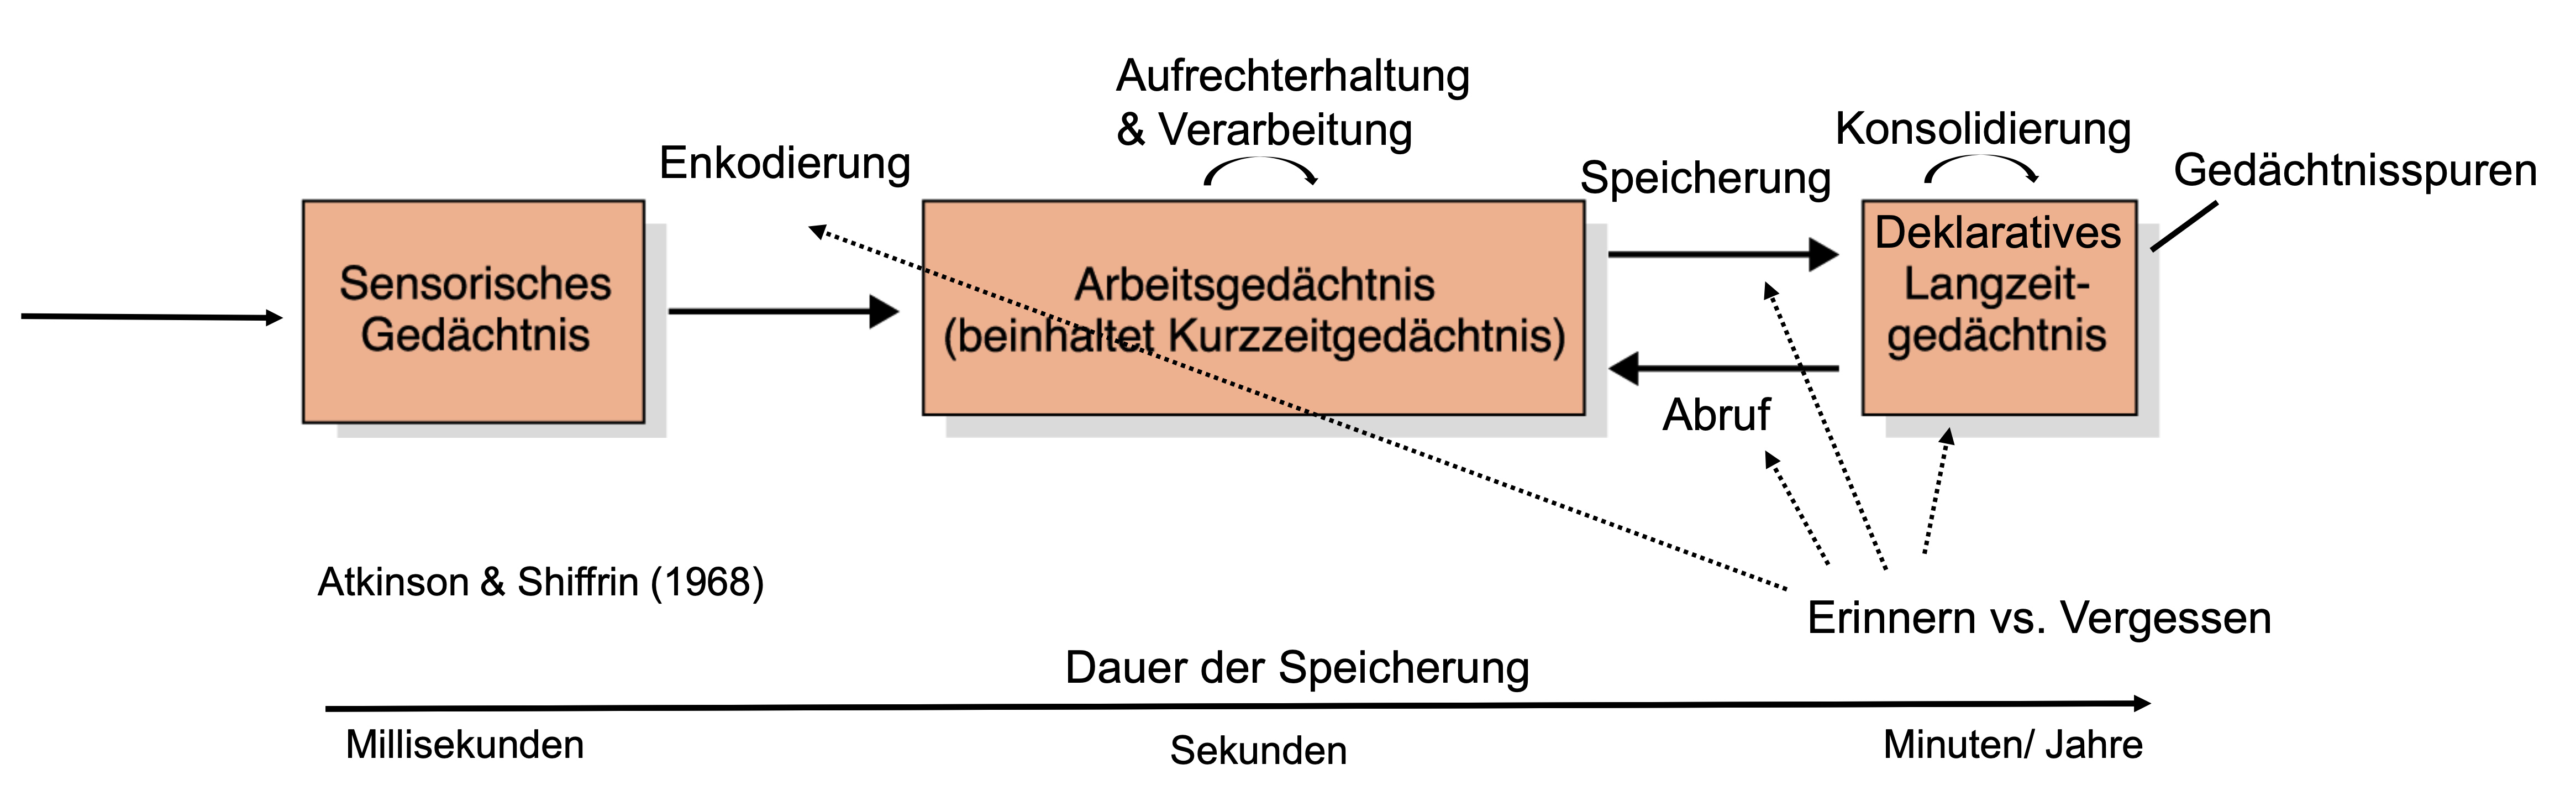
\includegraphics[scale=.2]{img/Drei_Speicher.png}
\end{center}
\subsubsection{Strukturen im Langzeitgedächtnis}
\begin{center}
	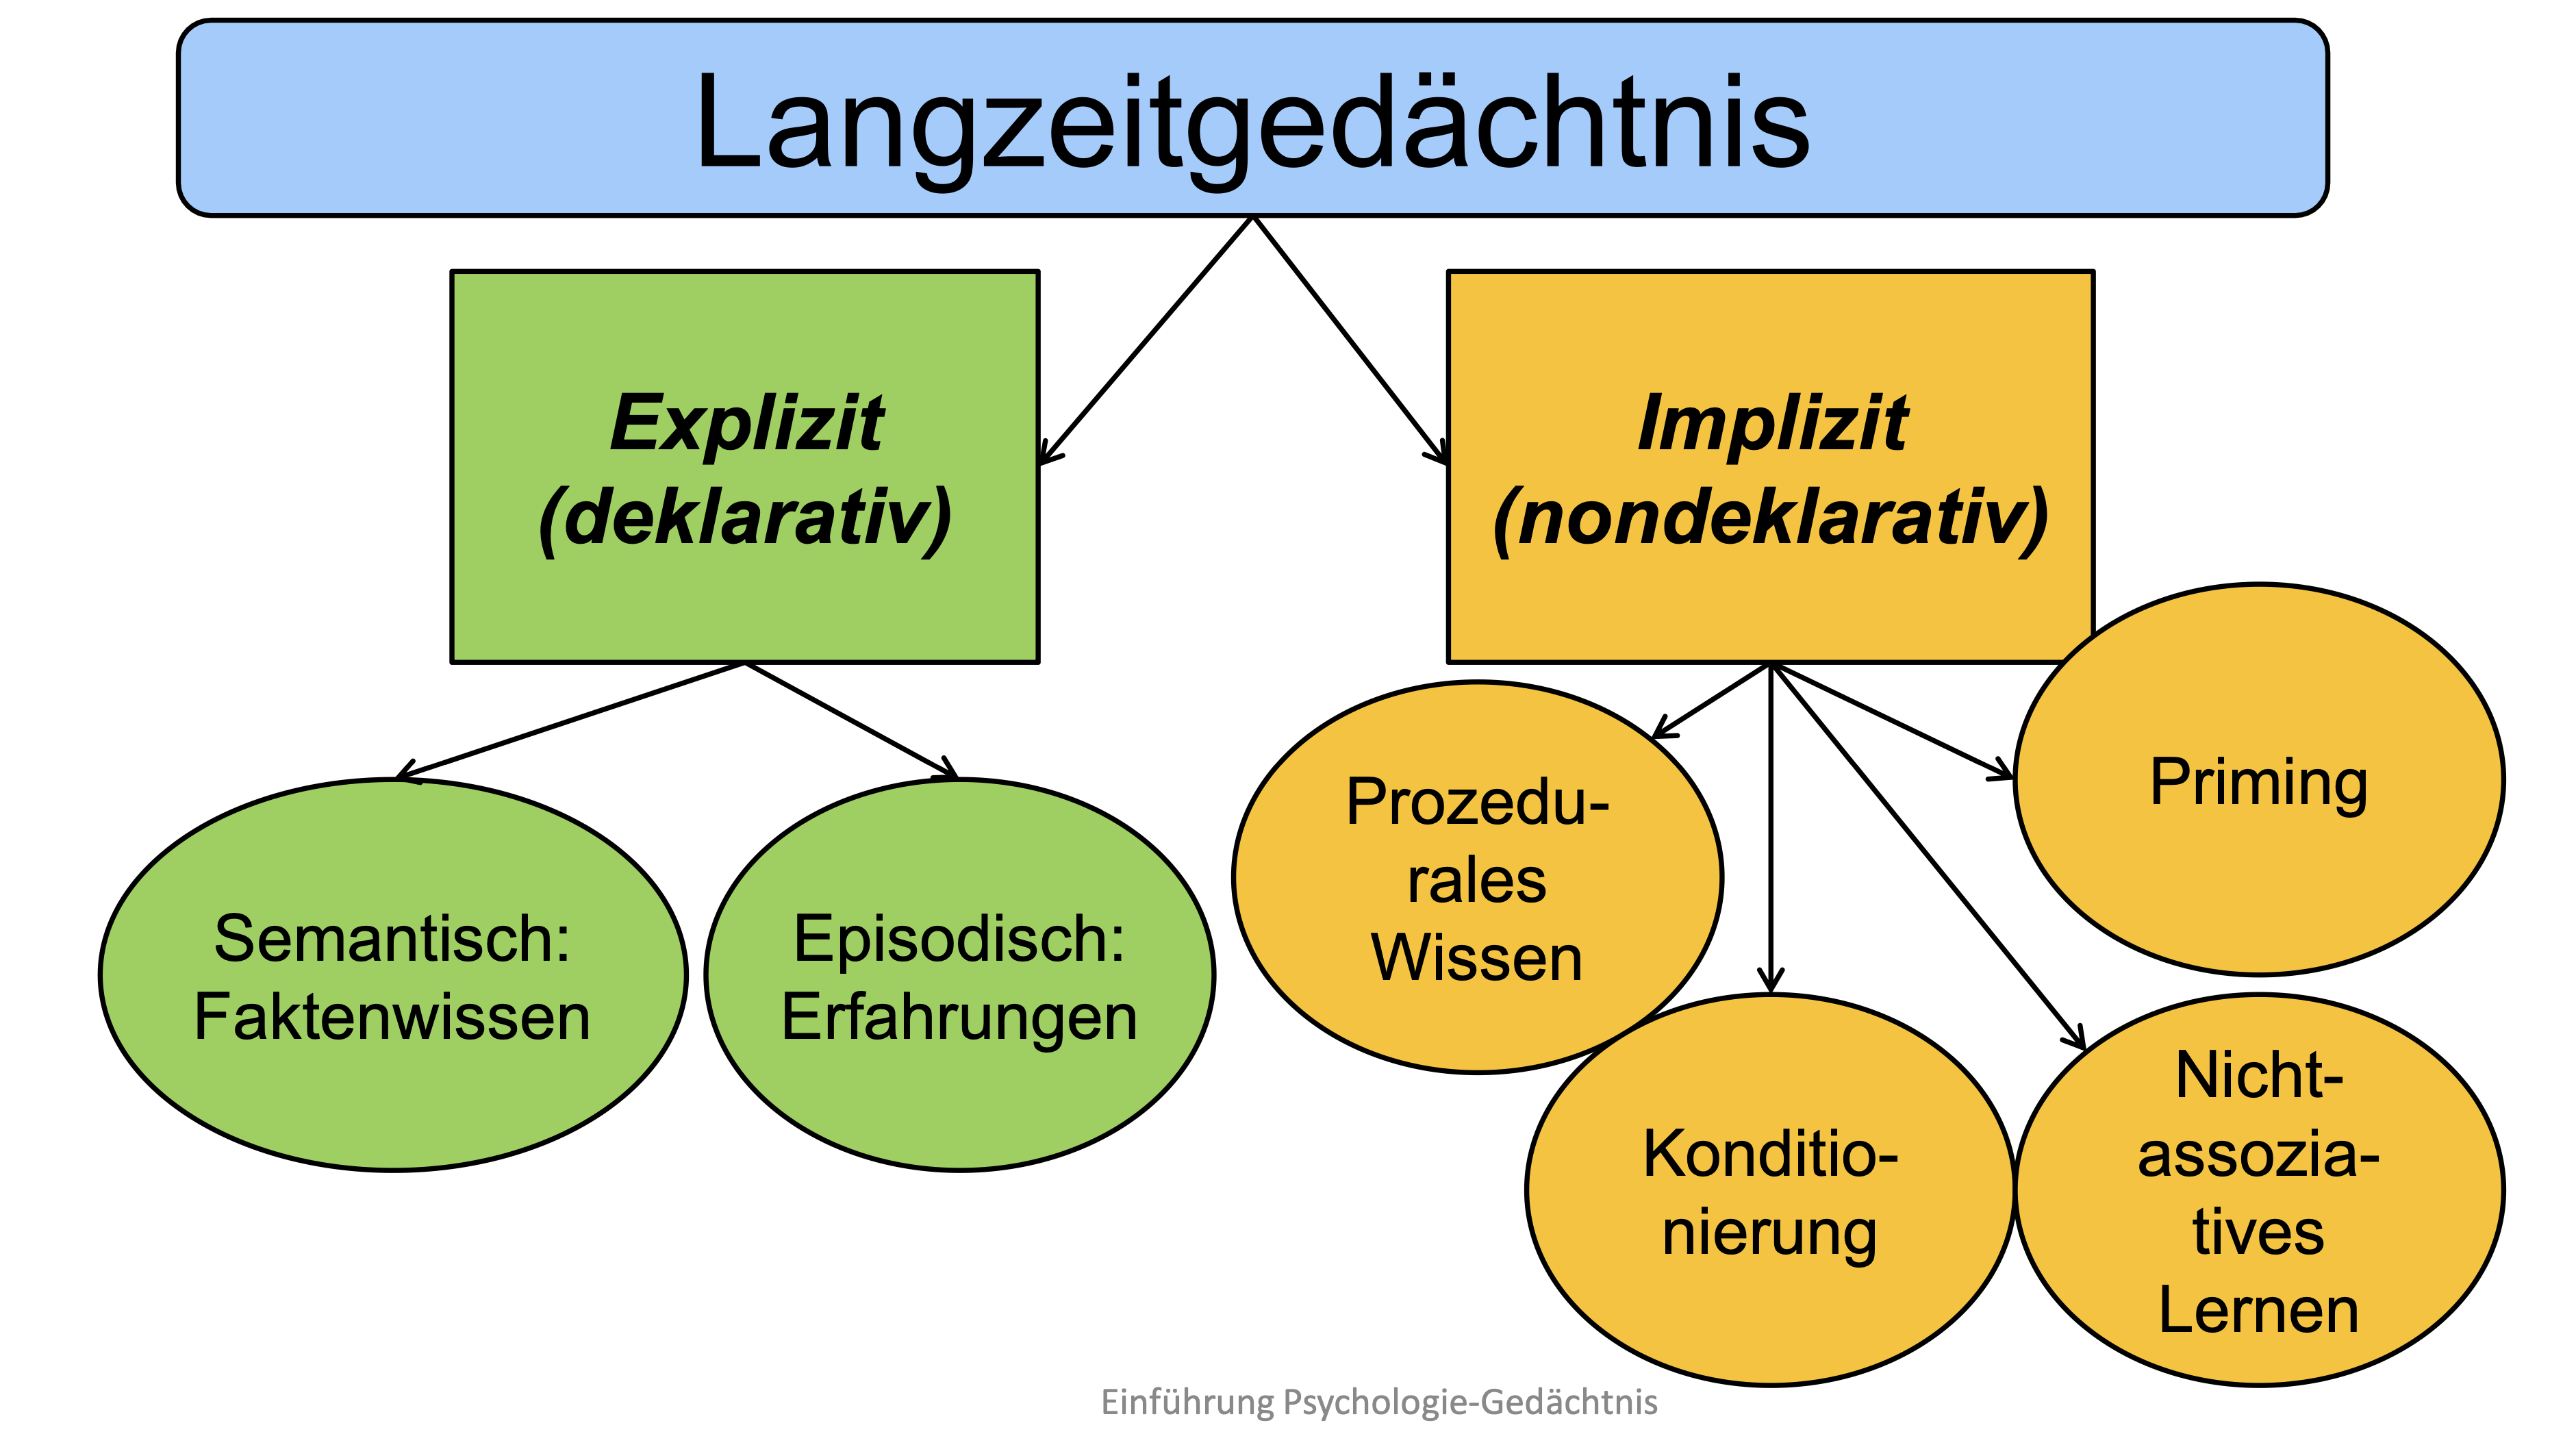
\includegraphics[scale=.2]{img/Langzeitgedaechtnis.png}
\end{center}
\subsubsection{Sensorisches Gedächtnis}
\begin{itemize}
	\item Ikonisches Gedächtnis:
		\begin{itemize}
			\item Sensorisches Gedächtnis für visuelle Informationen, speichert große Informationsmengen für sehr kurze Dauer (<500 ms)  
		\end{itemize}
	\item Echoisches Gedächtnis:
		\begin{itemize}
			\item Sensrisches Gedächtnis für auditive Informationen, speichert mit kurzer Dauer (<4 s) 
		\end{itemize}	
\end{itemize}
\subsubsection{Kurzzeitgedächtnis}
\begin{itemize}
	\item KZG: Gedächtnisprozesse, die die Repräsentation kürzlich enkodierter Erfahrungen aufrecht erhalten und Informationen aus dem Langzeitgedächtnis abrufen
	\item KGZ hat begrenzte Kapazität ($7\pm2$ Items) und speichert Informationen nur kurze Zeit (15-20 s)
	\item Trotz begrenzter Kapazität kommen wir im Alltag gut zurecht, dank:
		\begin{itemize}
			\item Rehearsal: Aufrechterhaltung durch mentale Wiederholung
			\item Chunking: Zusammenfassung in größere Sinneinheiten (chunks)
		\end{itemize}
\end{itemize}
\subsubsection{Arbeitsgedächtnis}
\begin{itemize}
	\item Arbeitsgedächtnis speichert und manipuliert mit begrenzter Kapazität Informationen für komplexe Aufgabenwie Verstehen, Lernen und Schlussfolgern
\end{itemize}
\subsubsection{Langzeitgeächtnis}
\begin{itemize}
	\item Assoziativität und Inhaltsadressierbarkeit:
		\begin{itemize}
			\item Abruf durch Hinweisreize (retrieval cues), die als Teil der Gedächtnisspur die gesamte Gedächtnisspur im LZG aktivieren
		\end{itemize}
	\item 2 Formen des expliziten Abrufs:
		\begin{itemize}
			\item Passives Wiedererkennen (recall)
			\item Aktiver Abruf (recall): Stimulus muss reproduziert werden
		\end{itemize}
	\item Enkodierspezifität:
		\begin{itemize}
			\item Abruf von Information wird in dem Maße besser, in dem die Hinweisreize beim Abruf mit den Umgebungsreizen beim Enkodieren übereinstimmen
		\end{itemize}
\end{itemize}
\subsubsection{Vergessen}
\begin{itemize}
	\item Vergessen: Verlust von Erinnerungen über die Zeit
	\item Interferenz: Ähnliche Gedächtnisspuren von alten und neuen Gedächtnisinhalten überlagern sich \rightarrow schlechterer Abruf von neuen und alten Inhalten 
\end{itemize}
\subsection{Neuronale Grundlagen des Gedächtnisses}
\begin{center}
	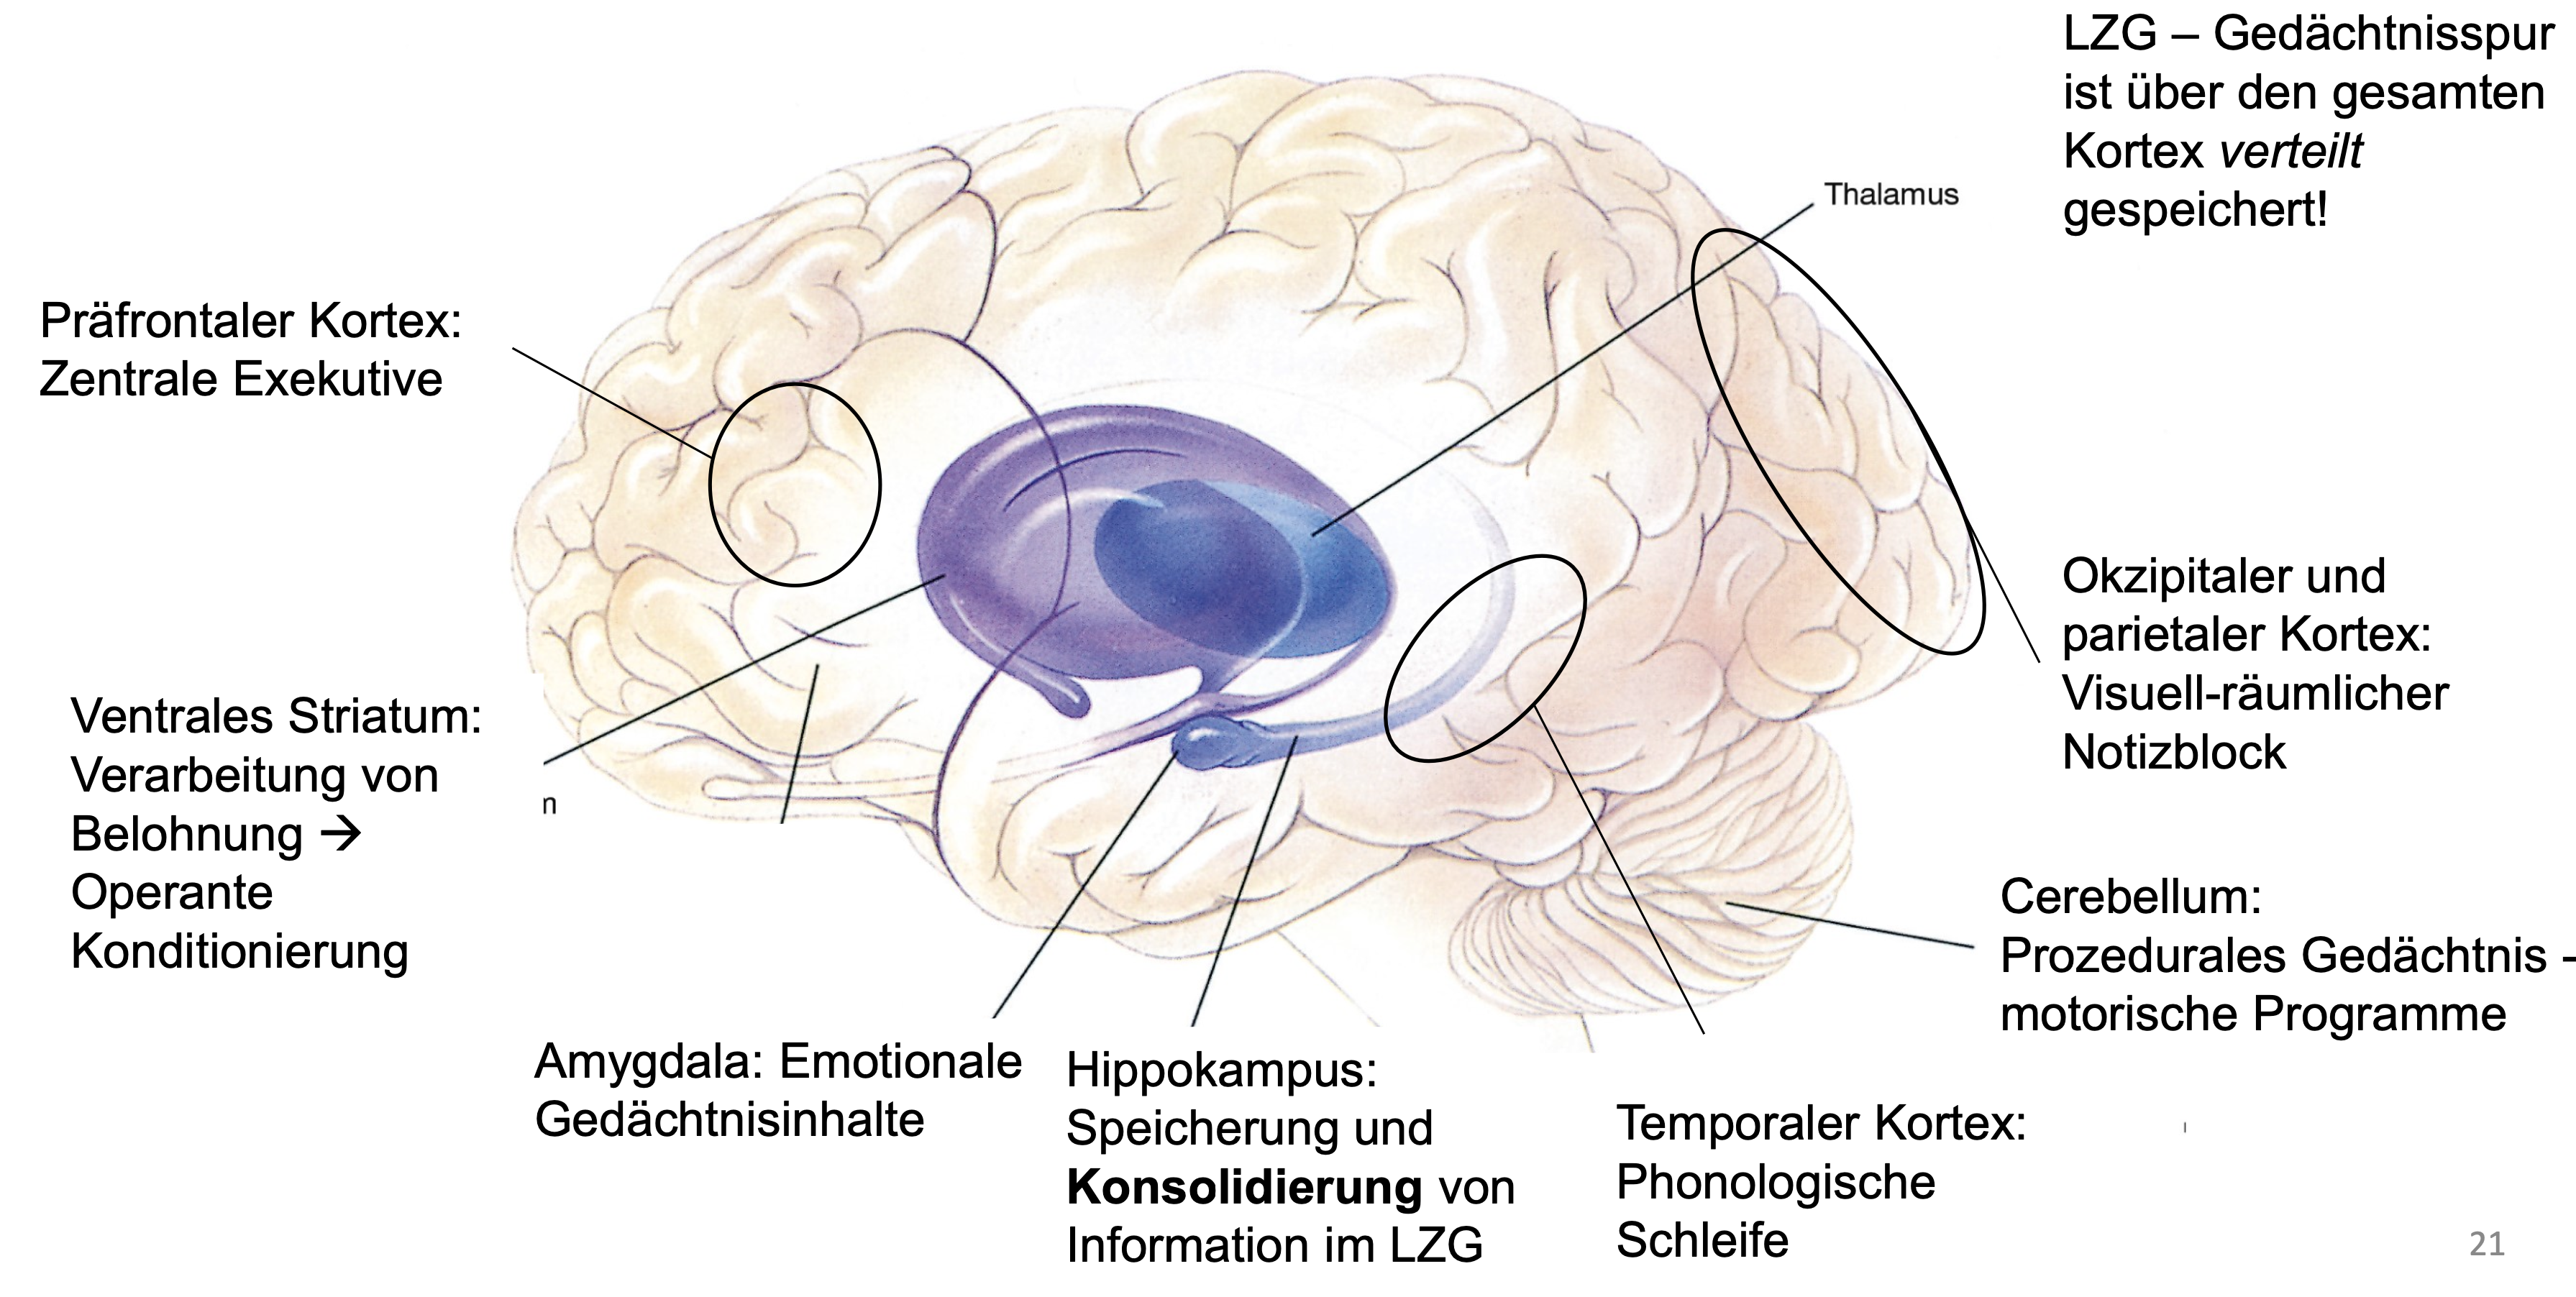
\includegraphics[scale=.2]{img/Gedeachtnis_Gehrin.png}
\end{center}
\subsubsection{Amnesien}
\begin{itemize}
	\item Anterograde vs. Retrograde Amnesie
		\begin{itemize}
			\item Anterograd: Unfähigkeit, neue Informationen nach Trauma/Krankheit zu speichern
			\item Retrograd: Unfähigkeit alte Informationen vor dem Trauma/Krankheit abzurufen
		\end{itemize}
	\item Amnesie bei
		\begin{itemize}
			\item Hirnschädigung: Entfernung des Hippokampus \rightarrow anterorage Amnesie mit intaktem KZG
			\item Demenzen, z.B. Alzheimer: Ablagerung von plaques beginnend im Hippokampus \rightarrow beide Arten der Amnesie
		\end{itemize}
\end{itemize}



\section{Kognition}
\begin{itemize}
	\item Allgemeinpsychologische Prozesse der Informationsgewinnung, -verarbeitung, und – nutzung, einschließlich Wahrnehmung, Aufmerksamkeit, Gedächtnis, Wissen, Sprache, Entscheiden, Problemlösen, logisches Denken etc.
	\item Kognitive Prozesse sind nicht direkt beobachtbar, sondern müssen aus Verhalten bzw. Gehirnaktivität erschlossen werden!
	\item Kognition $\not=$ Bewusstsein, da viele kognitive Prozess implizit sind
	\item Intelligenz: Individuelle Fähigkeit, mit seinen kognitiven Prozessen Probleme zu lösen  
\end{itemize}
\subsection{Methodischer Ansatz}
Vermessung kognitiver Prozesse durch Vergleich von Reaktionszeit. z.B. Farben und Nabe der Farbe trennen.

Der Reaktionszeitunterschied zwischen den automatischen (impliziten) Prozessen und Kontrollierten (expliziten) Prozessen kann auf kognitive Prozess schließen
\subsection{Sprachverständnis und Sprachproduktion}
Sprache: System der Kommunikation, dass Laute (Phoneme) und Schriftzeichen (Grapheme) nach grammatikalischen Regeln (Syntax) benutzt, um Gedanken, Erfahrungen, Ideen und Gefühle etc. (Bedeutung/Semantik) durch Wörter (Lexikon) auszutauschen
\subsubsection{Zentrale kognitive Prozesse der Sprache}
\begin{itemize}
	\item Sprachproduktion: Kognitive Prozesse, durch die wir Bedeutung symbolisch, z.B. durch Sprachlaute, ausdrücken
		\begin{itemize}
			\item Übersetzung von Gedanken (Bedeutung/Semantik) in Wörter (Lexikon) und Sätze nach grammatikalischen Regeln (Syntax) mit bestimmten Lauten (Phoneme)
			\item Hörerbezug: Abstimmung der Äußerung auf die Hörerschaft, für die sie gedacht ist (Pragmatik).
		\end{itemize}
	\item Sprachverständnis: Kognitive Prozesse, durch die wir die Bedeutung von sprachlichen Äußerungen erfassen
		\begin{itemize}
			\item Laute werden als Wörter wahrgenommen, deren Bedeutung zusammen mit der Syntax die Bedeutung des Satzes ergibt
			\item Schwierigkeit: Lexikalische und syntaktische Mehrdeutigkeit
		\end{itemize}
\end{itemize}
\subsubsection{Kognitive Prozesse beim Sprechen}
\begin{enumerate}
	\item Semantische Ebene
	\item Lexikalische Ebene
	\item Syntaktische Ebene
	\item Phonologische Ebene: Wegstabenverbuchseln
\end{enumerate}
\subsubsection{Mehrdeutigkeit beim Sprachverständnis}
Reihenfolge des Sprachverständnisses umgekehrt zum Sprechen
\subsection{Problemlösen und schlussfolgerndes Denken}
\begin{itemize}
	\item Induktives Schlussfolgern:
		\begin{itemize}
			\item Generalisierendes Schlussfolgern aus einzelnen Beobachtungen 
		\end{itemize}
	\item Deduktives Schlussfolgern:
		\begin{itemize}
			\item Spezifische Schlussfolgerung aus einer Prämisse/Hypothese
		\end{itemize}
\end{itemize}
\subsubsection{Induktives Schlussfolgern: Kognitive Heuristiken und Verzerrungen}
Induktive Schlüsse im Alltag:
\begin{itemize}
	\item Verfügbarkeitsheuristik: Ereignisse, an die wir uns leichter erinnern können, halten wir für wahrscheinlicher
	\item Repräsentativitätsheuristik: Objekte/Ereignisse/ Personen werden wahrscheinlicher einer Kategorie zugeordnet, wenn sie repräsentativ für die Kategorie erscheinen
	\item Bestätigungsverzerrung: Menschen suchen vor allem bestätigende Information und nehmen diese selektiv wahr!
\end{itemize}
\subsection{Intelligenz und Intelligenzdiagnstik}
\subsubsection{Psychometrische Intelligenztheorien}
\begin{enumerate}
	\item g-Faktorentheorie: Ein übergeordneter g-Faktor (Allgemeine Intelligenz) erklärt gut die Leistungen über verschiedene kognitive Fähigkeitstests hinweg
	\item Zweifaktorentheorie: Kristalline und Fluide Intelligenz
	\item Dreischichtenmodell: Vereint und erweitert I. \& II.
\end{enumerate}
\subsubsection{Intelligenzdiagnostik}
ProbandIn bearbeitet Aufgaben, die spezifische kognitive
Fähigkeiten erfassen: Schnelligkeit vs. Niveau. Vergleich mit Normstichprobe im gleichen Alter \rightarrow IQ







\section{Entwicklung}
\end{document}